\chapter{Desarrollo del Software} \label{ch:softwareDevelopment}

% **************************** Define Graphics Path **************************
\ifpdf
    \graphicspath{{Chapter4/Figs/Raster/}{Chapter4/Figs/PDF/}{Chapter4/Figs/}}
\else
    \graphicspath{{Chapter4/Figs/Vector/}{Chapter4/Figs/}}
\fi

En este capítulo se detalla el comportamiento del software ad-hoc implementado para este trabajo. El mismo se encuentra dividido en dos secciones, en la primera se detalla la estructura del simulador de todo el sistema, el cual fue realizado tanto para realizaciones de pruebas de concepto como comparaciones de como se degradan los resultados de un sistema real comparado a un escenario ideal. La segunda detalla la estructura y funcionamiento del procesador de señales utilizado para el radar. El desarrollo de ambas aplicaciones de software se basó en la teoría descrita en el capítulo \ref{ch:theory}. Por último, en las explicaciones se hace uso de diagramas de clase y secuencia.

\section{Simulador}

El simulador se realizó para estudiar y poder determinar cuáles son los factores que mayormente afectan a las mediciones y funcionamiento del radar. Para ello se incluyeron algunas fuentes de incertidumbre, colocándolas como configurables para ensayar sus consecuencias de forma individual. Cabe destacar que el lenguaje utilizado para el desarrollo fue python 3 \cite{python3}.

Los parámetros de configuración para realizar una corrida se listan en la tabla \ref{tab:simulatorParameters}.

\begin{table}[htb]
  \caption{Parámetros de configuración utilizados en el simulador.}
  \centering
  \label{tab:simulatorParameters}
  \begin{tabular}{l l l}
  \toprule
  \textbf{Subsistema} & \textbf{Parámetro} & \textbf{Notas} \tabularnewline
  \midrule
  \multirow{6}{2cm}{Señal Transmitida} & BW & Ancho de banda en $\si{\hertz}$ \tabularnewline

   & F0 & Frecuencia central en $\si{\hertz}$ \tabularnewline

   & FS & Frecuencia de muestreo en $\si{\hertz}$ \tabularnewline

   & T & Período en $\si{\second}$ \tabularnewline

   & P & Potencia en $\si{\deci\bel}$ \tabularnewline

   & $\varphi$ & Fase inicial en $\si{\radian}$ \tabularnewline
  \cmidrule{2-3}
  \multirow{2}{*}{Blanco} & Phase & Desfase en $\si{\radian}$ introducido por el blanco en la señal \tabularnewline

   & Gain & Ganancia en $\si{\deci\bel}$ introducida por el blanco en la señal \tabularnewline
  \cmidrule{2-3}
  \multirow{5}{*}{Radar} & FS & Frecuencia de muestreo en $\si{\hertz}$ del receptor \tabularnewline

   & $G_tG_r$ & Ganancia de transmisión y recepción de las antenas. \tabularnewline

   & Range & Distancia en $\si{\meter}$ entre el blanco y el radar \tabularnewline

   & $\Delta Range$ & Distancia en $\si{\meter}$ entre el medidor de rango y el mezclador \tabularnewline

   & std Range & Desvío estándar en $\si{\meter}$ del medidor de rango \tabularnewline
  \bottomrule 
  \end{tabular}
\end{table}

Las figura \ref{fig:classDiagramSimulator} y \ref{fig:sequenceSimulator} muestran el diagrama de clases del simulador y la secuencia de ejecución para obtener la ganancia y desfase que el blanco induce sobre la señal transmitida por el radar. Los mismos fueron realizados siguiendo la nomenclatura UML \cite{uml2.5}.

\begin{figure}[H]
 \centering
 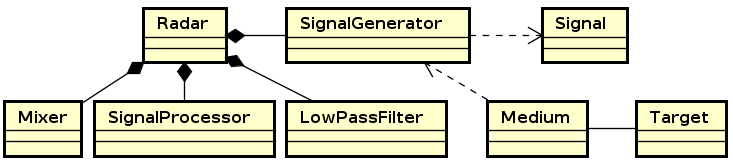
\includegraphics[width=12cm]{classDiagramSim}
 \caption{Diagrama de clases del simulador.}
 \label{fig:classDiagramSimulator}
\end{figure}
En la figura \ref{fig:classDiagramSimulator} se pueden identificar varias clases a definir.
\begin{itemize}
  \item Radar: Esta clase simula el comportamiento del radar, el cual está compuesto por los siguientes subsistemas:
  \begin{itemize}
    \item Mixer: Este es el mezclador, el cual multiplica la señal recibida con la señal transmitida.
    \item LowPassFilter: Esta clase es el pasa bajos, el cual filtra la señal mezclada para eliminar las altas frecuencias.
    \item SignalProcessor: Esta clase es el procesador de la señal, es la encargada de obtener la ganancia y desfase que el blanco introduce a la señal propagada por el medio.
    \item SignalGenerator: Es el generador de la señal a transmitir.
  \end{itemize}

  \item Signal: Es la clase que representa las distintas posibles señales en todo el sistema.
  \item Medium: Es el medio que atenúa y desfasa la señal en función a la distancia de propagación.
  \item Target: Es el blanco, el cual genera el eco desfasado y con cierta ganancia con respecto a la señal incidente.
\end{itemize}

\begin{figure}[htb]
 \centering
 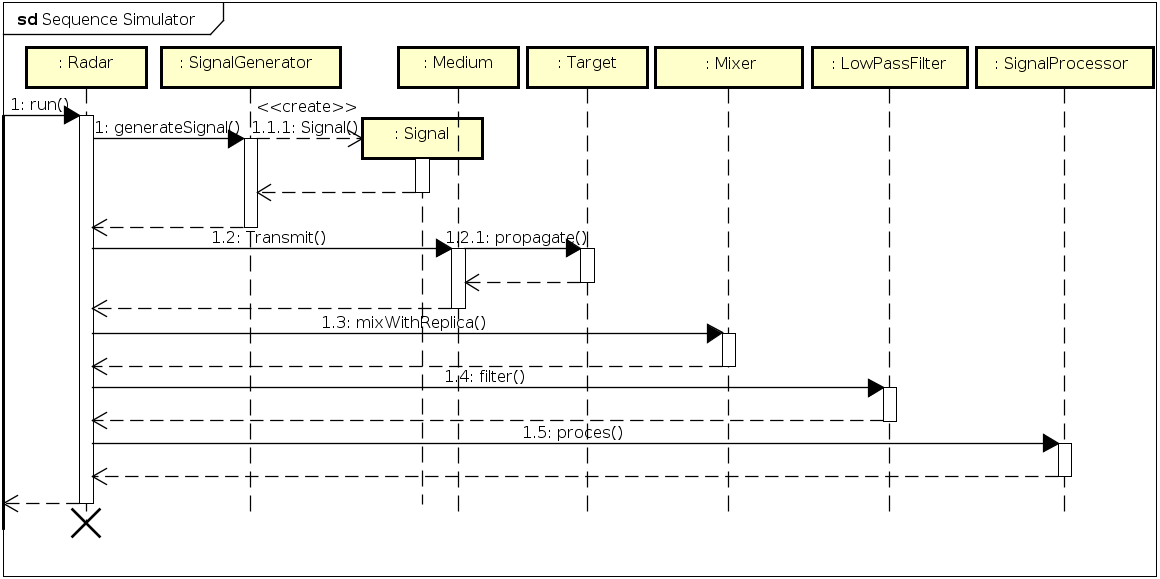
\includegraphics[width=15cm]{sequenceSimulator}
 \caption{Diagrama de secuencia del simulador para obtener la ganancia y fase del blanco.}
 \label{fig:sequenceSimulator}
\end{figure}
La secuencia de ejecución que se muestra en la figura \ref{fig:sequenceSimulator} se la interpreta de la siguiente manera. El radar utiliza el generador de señales para generar la chirp a transmitir, la cual se propaga por el medio hasta el blanco. En el blanco se produce un eco que también se propaga por el medio hasta ser recibido por la antena receptora del radar. La señal recibida pasa por dos subsistemas previamente a ser procesada, el primero es el mezclador que la multiplica con una replica y el segundo es un pasa bajos. El procesador obtiene la fase y ganancia introducidos por el blanco.

\section{Procesador de señales del Radar} \label{sc:radarProcessor}

El procesador de señales, a parte de obtener la fase y ganancia del blanco iluminado, determina la distancia a la que está el mismo, la potencia de la señal recibida y la potencia y desfase que el medio introduce sobre la señal. Para ello, se desarrolló una aplicación que utiliza el conector del micrófono de la computadora como receptor.

Es necesario que la computadora tenga un conector dedicado porque se utilizan ambos canales del mismo. En uno se recibe la señal de sincronización para poder determinar el período de la chirp transmitida y en el otro se recibe la señal mezclada y filtrada por el pasa bajos. Es importante que se procesen ambas señales a la vez dado que las mismas se encuentran sincronizadas, de otra forma no se podría determinar a priori que parte de la señal recibida se corresponde al período de uno u otro pulso transmitido.

En la sección \ref{sc:ambiguity} se discutió sobre la ambigüedad de rango en los radares FMCW y que hay que descartar la sección inicial y final del período para eliminar frecuencias indeseadas, dependiendo del tiempo de ida y vuelta de la señal transmitida, por ende de la distancia a la que se encuentra el blanco iluminado. 

En el desarrollo del radar, no es necesario eliminar dicha sección dado que, para la mayor frecuencia de muestreo del micrófono, $\SI{40}{\kHz}$, y el rango máximo de medición del blanco, que ronda alrededor de los $\SI{15}{\m}$, el cálculo da que la fracción de señal a eliminar es menor a 1 muestra.

Los parámetros de configuración del procesador de señales se listan en la tabla \ref{tab:radarParameters}.

\begin{table}[htb]
  \caption{Parámetros de configuración del receptor.}
  \centering
  \label{tab:radarParameters}
  \begin{tabular}{l l p{9cm}}
  \toprule
  \textbf{Parámetro} & \textbf{Default} & \textbf{Notas} \tabularnewline
  \midrule
  Real Time & True & Determina si la entrada es desde el jack del micrófono (True) o un archivo de audio (False). \tabularnewline

  Measure Phase & True & Grafica la frecuencia de la señal recibida o el histograma de la fase. \tabularnewline

  Min Freq & $\SI{200}{\hertz}$ & Frecuencia mínima para buscar el pico de la señal. \tabularnewline

  Max Freq & $\SI{800}{\hertz}$ & Frecuencia máxima a ser graficada. \tabularnewline

  Spec Len & 100 & Longitud en tiempo del espectrograma. \tabularnewline

  Tx power & $\SI{11.87}{\dBm}$ & Potencia transmitida por el radar. \tabularnewline

  Ganancia Antenas & $9$ & Multiplicación de las ganancias de las antenas transmisora y receptora. \tabularnewline
  \bottomrule 
  \end{tabular}
\end{table}

Las figura \ref{fig:RadarsClassDiagram} y \ref{fig:radarsSequence} muestran el diagrama de clases del procesador y la secuencia de ejecución para obtener la ganancia y desfase que el blanco induce sobre la señal transmitida por el radar. Los mismos fueron realizados  siguiendo la nomenclatura UML \cite{uml2.5}.

\begin{figure}
 \centering
 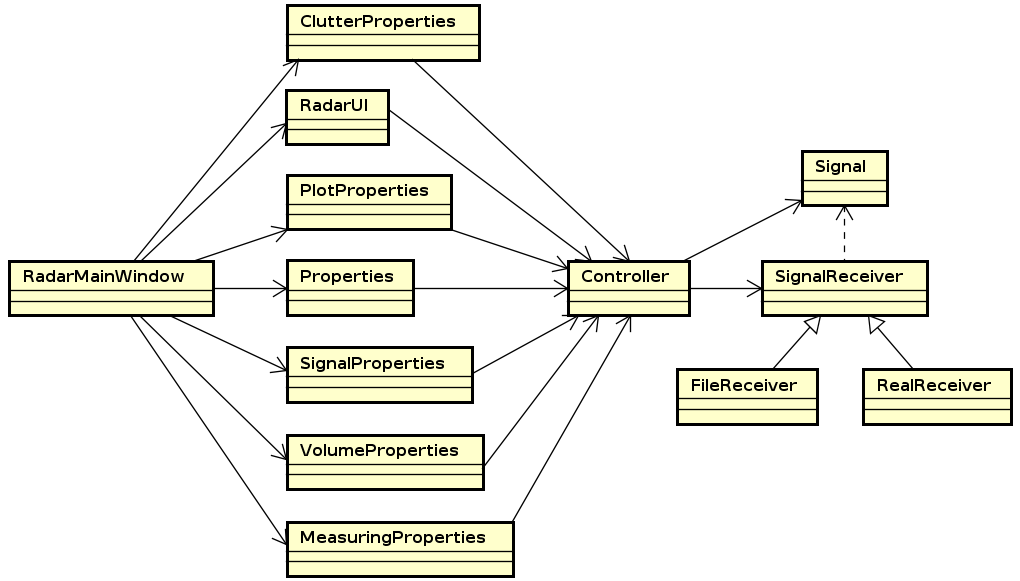
\includegraphics[width=12cm]{classDiagramRadar}
 \caption{Diagrama de clases del procesador de señales.}
 \label{fig:RadarsClassDiagram}
\end{figure}
En la figura \ref{fig:RadarsClassDiagram} se pueden identificar varias clases a definir.
\begin{itemize}
  \item RadarMainWindow: Esta clase se corresponde a la ventana principal y solamente posee el manejo de los botones de cierre y minimización del programa.
  \item ClutterProperties: En esta clase se puede restar a la señal recibida el clutter medido, tanto de la misma adquisición como de un archivo externo.
  \item RadarUI: Esta clase es la encargada de mostrar los distintos gráficos. Dichos gráficos muestran la tensión del pulso recibido durante un período de transmisión. A su vez muestra un histograma de fase medida y de distancia detectada a la que se encuentra el blanco. Con esta clase se cumple el requerimiento \ref{req:l2_plots}.
  \item PlotProperties: En esta clase se configura que gráfico se desea mostrar en pantalla, si el histograma de fase o la FFT de la señal recibida.
  \item Properties: En esta clase se muestran las mediciones con sus incertidumbres de las propiedades del blanco y de la señal recibida. Con esta clase se cumple el requerimiento \ref{req:l2_measurements}.
  \item SignalProperties: En esta clase se puede cargar la señal a procesar desde un archivo. A su vez se puede pausar, iniciar, rebobinar y rebobinar automáticamente la pista de audio. También se puede seleccionar el modo tiempo real. Con esta clase se cumple el requerimiento \ref{req:l2_realTime}.
  \item VolumeProperties: En esta clase se puede modificar la señal recibida en los decibeles deseados.
  \item MeasuringProperties:  En esta clase se pueden reiniciar el cálculo de las incertidumbres de los parámetros medidos. A su vez, se puede introducir la distancia entre el blanco y el radar medido por un instrumento externo.
  \item Controller: Esta clase es la encargada de procesar la señal recibida y reportar los resultados obtenidos.
  \item Signal: Es la clase que representa las distintas posibles señales en todo el sistema.
  \item SignalReceiver: Esta clase es la encargada de tomar una cantidad de muestras de la señal a procesar. Es la generalización de las siguientes clases:
  \begin{itemize}
    \item FileReceiver: Esta clase utiliza como entrada un archivo de audio.
    \item RealReceiver: Esta clase utiliza como entrada el micrófono de la computadora.
  \end{itemize}
\end{itemize}

\begin{figure}[htb]
 \centering
 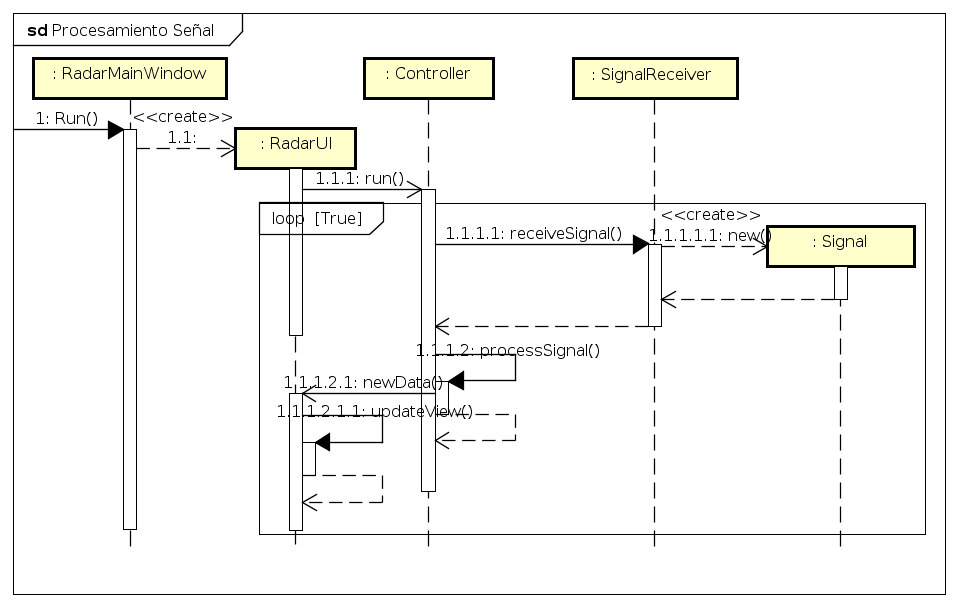
\includegraphics[width=15cm]{sequenceRadar}
 \caption{Diagrama de secuencia del radar para obtener la ganancia y fase del blanco.}
 \label{fig:radarsSequence}
\end{figure}
La secuencia de ejecución que se muestra en la figura \ref{fig:radarsSequence} se la interpreta de la siguiente manera. Independientemente de donde se configure la entrada de la señal, la clase signalReceiver toma una cantidad de muestras del flujo de datos, crea la clase señal y se la otorga al controlador para procesarla. En dicho procesamiento se obtiene la ganancia y desfase del objeto iluminado, para ello se mide el pico de frecuencia para determinar la distancia del blanco, se le resta la potencia de transmisión y la atenuación que el medio introduce sobre la misma. Todos los resultados se reportan en la GUI (clase RadarUI).

\begin{figure}[htb]
 \centering
 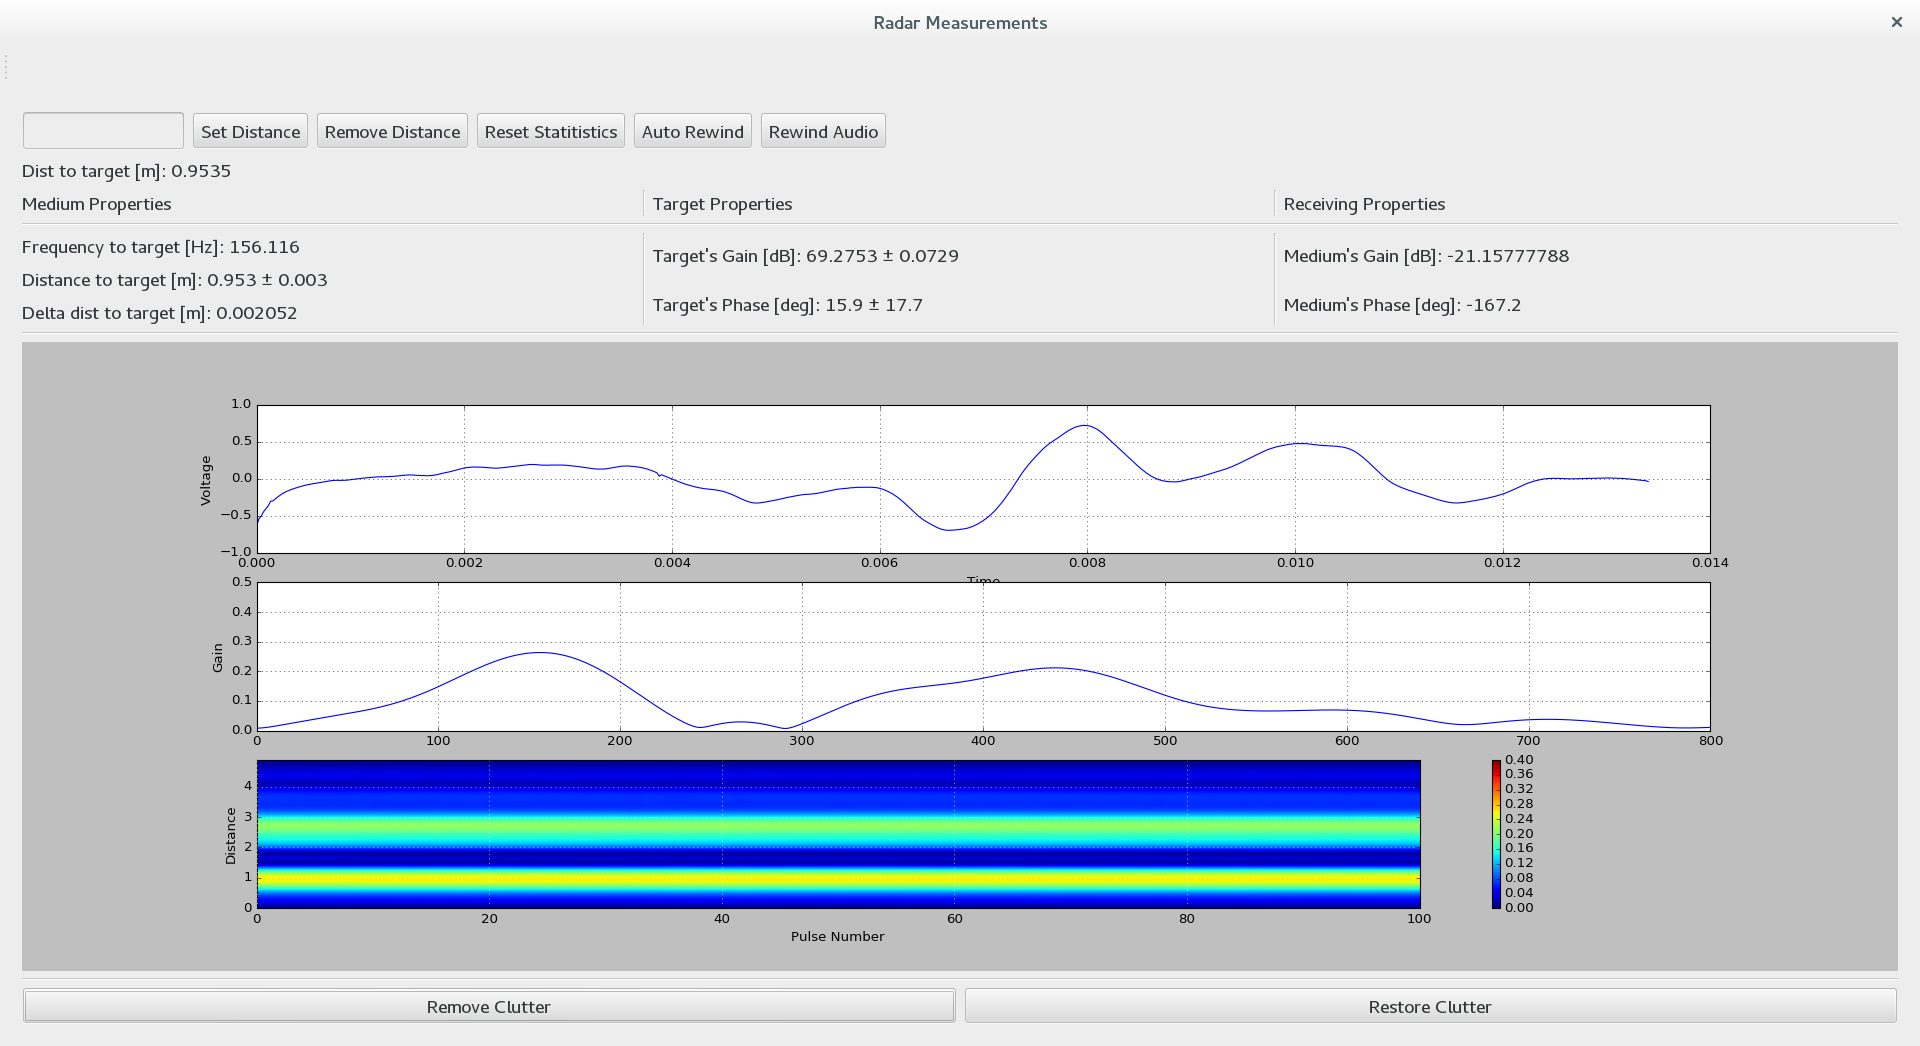
\includegraphics[width=15cm]{radarGUI}
 \caption{Interfaz gráfica del procesador de la señal del radar.}
 \label{fig:radarSnapshot}
\end{figure}
En la figura \ref{fig:radarSnapshot} se muestra la interfaz gráfica. Se puede observar que la misma posee 5 secciones con botones para diferentes funcionalidades, de esta forma se cumple el requerimiento \ref{req:l2_buttons}. El contenido de cada una se describe a continuación.
\begin{itemize}
  \item Sección "Signal Properties": Esta sección está compuesta por 4 botones.
  \begin{itemize}
    \item Botón "Browse": Con el mismo se puede seleccionar una pista de audio para ser procesada. Una vez cargada, la funcionalidad de dicho elemento se modifica para detener el análisis de la pista cargada.

    \item Botón "Play": Con el mismo se puede iniciar el análisis de la pista cargada. Durante el análisis, la funcionalidad de dicho elemento se modifica habilitando el pausado de la ejecución.

    \item Botón "Loop": Al presionar dicho elemento, se rebobina automáticamente la pista de audio al llegar al fin del archivo.
  \end{itemize}

  \item Sección "Volume Properties": Esta sección está compuesta por 4 botones y un textBox.
  \begin{itemize}
    \item TextBox: Dicho campo acepta un valor numérico que representa el volumen a aplicar a la señal recibida, en $\si{\dB}$.

    \item Botón "Set Volume": Al presionar dicho botón y, si el usuario introdujo un valor en el TextBox, el procesador de señales utiliza el volumen introducido para amplificar la señal recibida.

    \item Botón "Reset Volume": Al utilizar este botón, el valor introducido en el TextBox es removido y el procesador de señales vuelve a mostrar la señal recibida sin amplificar.

    \item Botón "Increase Volume": Este botón incrementa en $\SI{1}{\dB}$ el volumen de la señal recibida.

    \item Botón "Decrease Volume": Este botón decrementa en $\SI{1}{\dB}$ el volumen de la señal recibida.
  \end{itemize}

  \item Sección "Measurements Properties": Esta sección está compuesta por 3 botones y un textBox.
  \begin{itemize}
    \item Botón "Reset Statistics": Al utilizar este botón se reinician todas las incertidumbres obtenidas en las mediciones.

    \item TextBox: Dicho campo acepta un valor numérico que representa la distancia entre el radar y el blanco iluminado. El valor introducido por el usuario puede ser utilizado por el procesador de señales para la obtención de la fase y ganancia del blanco iluminado.

    \item Botón "Set Distance": Al hacer click en este botón y, si el usuario introdujo un valor en el TextBox, el procesador de señales utiliza la distancia introducida para el procesamiento de la señal recibida.

    \item Botón "Remove Distance": Al utilizar este botón, el valor introducido en el TextBox es removido y el procesador de señales vuelve a determinar la distancia entre el blanco iluminado y el radar a partir de la señal recibida.
  \end{itemize}

  \item Sección "Plot Properties": Esta sección está compuesta por 2 botones.
  \begin{itemize}
    \item Botón "Plot phase": Al utilizar este botón se grafica el histograma de fase del blanco medido por el radar.

    \item Botón "Plot FFT": Al utilizar este botón se grafica la FFT del blanco medida por el radar.
  \end{itemize}

  \item Sección "Clutter Properties": Esta sección está compuesta por 2 botones.
  \begin{itemize}
    \item Botón "Browse Clutter": Se puede seleccionar una pista de audio del clutter medido de la sala.

    \item Botón "Remove clutter": Si no se cargó una pista de audio con el botón "Browse Clutter", se guarda el estado de la señal recibida en el momento de presionar dicho botón. Las subsiguientes recepciones de datos son restados por este valor. En caso contrario, la señal recibida se resta con el estado de la señal cargada. Una vez presionado, la funcionalidad de dicho objeto se modifica para pausar el proceso en que se remueve el clutter.
  \end{itemize}
\end{itemize}


\section{Resumen}

En este capítulo se detalla el procesamiento de software realizado tanto para procesar la señal recibida por el radar como el simulador para validar el modelo matemático.

El simulador fue programado para realizar distintos ensayos para estudiar el impacto que tiene la adición de ciertos tipos de incertidumbres, ya sea como ruido en la señal transmitida como errores en la determinación de la distancia entre el radar y el blanco iluminado.

El receptor del radar puede recibir en dos modos principales, en tiempo real, recibiendo directamente del conector del micrófono de la computadora o leyendo desde una grabación de audio. Para ambos casos hay distintas funcionalidades para distintos tipos de ensayos, tales como introducir desde una fuente externa la distancia al blanco y la remoción de la señal del clutter.
